\section{Theoretische Grundlagen}
  
  Die High Performance Liquid Chromatography (HPLC) ist ein häufig verwendetes Trennverfahren. Die mobile Phase ist flüssig und durchströmt unter hohem Druck eine Säule, die die stationäre Phase enthält. Aufgrund von unterschiedlich starken Wechselwirkungen der in der mobilen Phase \textit{gelösten} Substanzen mit der stationären Phase kommt es zur Trennung. \citep{SkriptHPLC}\footnote{das ausgegebene Skript referenziert auf \citep{QuantitativeAnalyseHarris}, \citep{InstrumentelleAnalytikSkoog} und \citep{ModernLiquidChromatography} - im Folgenden wird aus Gründen der Einfachheit nur auf das Skript verwiesen}
  
  \subsection{Aufbau der HPLC und Ablauf einer Analyse}
    
    Eine HPLC besteht aus einer Vorrichtung zur Probenaufgabe, einer Vorrichtung zur Lagerung der Lösungsmittel inklusive Entgaser, einer Pumpe, einer Trennsäule, einem Detektor und einem Gerät zur Auswertung. Die einzelnen Bestandteile werden in Abbildung \ref{fig:AufbauHPLC} schematisch dargestellt. Der grundsätzliche Aufbau verändert sich bis auf die Trennsäule und den Detektor nicht. Diese können je nach Analyse ausgetauscht werden. 
    
      \begin{figure}[H]
        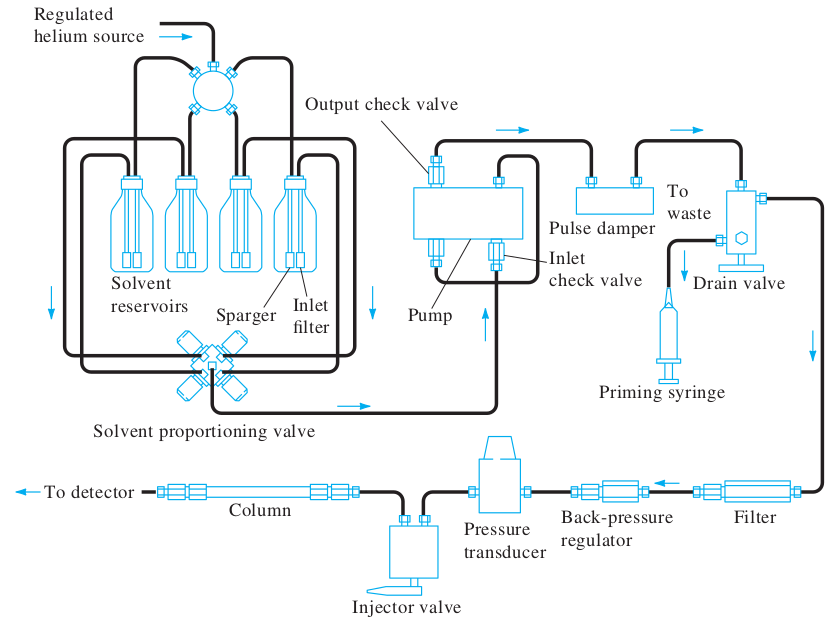
\includegraphics[scale=0.3, center]{images/PartsOfHPLC.png} 
        \caption[Schematischer Aufbau einer HPLC (Eigentum der PerkinElmer Corp., Norwalk, CT), Quelle: ]{Schematischer Aufbau einer HPLC (Eigentum der PerkinElmer Corp., Norwalk, CT).}
        \label{fig:AufbauHPLC}
      \end{figure}
    Im Folgenden werden die einzelnen Bestandteile näher beschrieben.
      
     \subsubsection{Probenaufgabe}
       
       Die Probenaufgabe erfolgt entweder manuell oder automatisch. Die manuelle Aufgabe wird heutzutage hauptsächlich bei präparativen Trennung verwendet. Bei der üblichen automatischen Aufgabe erfolgt die Injektion mit einer Spritze über ein 6-Wege Ventil. \citep{SkriptHPLC}
       
         \begin{figure}[H]
           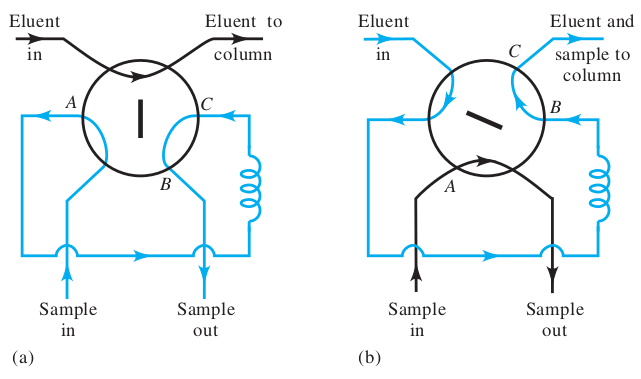
\includegraphics[scale=0.3, center]{images/Funktionsweise6WegeVentil.png} 
           \caption[Beschreibung der Funktionsweise des 6-Wege Ventil, Quelle: ]{6-Wege Ventil: in Position (a) wird die Probenschleife ACB gefüllt, in Position (b) wird die Probe mithilfe des Eluenten in die Säule überführt}
           \label{fig:SechsWegeVentil}
         \end{figure}
         
     \subsubsection{Lösungsmittel und Entgaser}
       
       Häufig wird eine Mischung aus mehreren Lösungsmittel benötigt, um die Polarität der mobilen Phase besser einstellen zu können. Die Zusammensetzung wird über ein Ventil reguliert. Der Entgaser entfernt die restlichen Gasteilchen der Laufmittel, da diese die Messung beeinträchtigen können. \citep{InstrumentelleAnalytikSkoog}
       
     \subsubsection{Pumpe}
     
     \subsubsection{Trennsäule}
     
     \subsubsection{Detektor}
     
  \subsection{Trennmechanismen}
    
  \subsection{Chromatographische Parameter}
    
    Um den Trennvorgang sowie die Trennleistung einer Analyse bzw. einer Säule zu charakterisieren, hat sich eine Vielzahl an Kenngrößen und Parametern etabliert, die im Folgenden beschrieben werden.
    
     Um die Position und das Aussehen eines Peaks zu beschreiben eignet sich die Totzeit $t_0$ (Zeit der Probe in der mobilen Phase), die Bruttoretentionszeit $t_B$ (Zeit der Probe in mobiler und stationärer Phase), die Nettoretentionszeit $t_R$ (Zeit der Probe in der stationären Phase - $t_R = t_B - t_0$), die Basispeakbreit $w$ (Anlegen zweier Tangenten in \SI[mode=text]{60}{\percent} Peakhöhe und Bestimmung des Abstandes der Schnittpunkte mit der Basislinie) und die Peaksymmetrie. 
    
    Wechselwirkungsvorgänge werden durch den Kapazitätsfaktor $k$ (relative Verweildauer des Analyten in stationärer Phase - $k = t_R / t_0$), den Verteilungskoeffizient $K$ ($K = c_S / c_M$ in Analogie zum Massenwirkungsgesetz) und die lineare Strömungsgeschwindigkeit $v$ ($v = L / t_R$ mit Säulenlänge $L$) beschrieben. 
    
    Die Effizienz einer Trennsäule wird durch die theoretische Trennstufenhöhe (Bodenhöhe) $H$ und die Anzahl an theoretischen Böden (Trennstufenzahl) $N$ charakterisiert ($L = N H$). Die Anzahl an theoretischen Böden ist ein Maß für die Anzahl an theoretischen Gleichgewichtseinstellungen des Analyten zwischen mobiler und stationärer Phase und kann u. a. mit 
    
      \begin{equation}
        N = 16 \left(\frac{t_R}{w}\right)^2
      \end{equation} 
    unabhängig von $H$ und $L$ berechnet werden. Die Bodenhöhe in Abhängigkeit von der linearen Strömungsgeschwindigkeit $v$ wird durch die Van-Deemter Gleichung 
    
      \begin{equation}
        H(v) = A + \frac{B}{v} + C v
      \end{equation}
    beschrieben (Beiträge der Eddy-Diffusion $A$, Longitudinaldiffusion $B$ und des verzögerten Massentransfers $C$). \textit{Bild einfügen} Die maximale Trennleistung erfolgt am Minimum der Kurve. 
    
    Die Trennleistung, also die Fähigkeit zwei benachbarte Peaks eindeutig aufzutrennen, wird durch die Auflösung $R = 2\left(t_{R2} - t_{R1}\right) / \left(w_2 + w_1\right)$ und die relative Retention bzw. Selektivität $\alpha = t_{R2} / t_{R1}$ charakterisiert. Desto größer $R$ und $\alpha$ sind, desto  besser ist die Trennung. \citep{Versuchsvorschrift}
    
  \subsection{Kalibrierung über einen internen Standard}
  
    Man benötigt einen Standard, der ähnliche physikalische und chemische Eigenschaften wie die Probe besitzt. Zur Kalibrierung werden mehrere Lösungen mit jeweils gleicher Standardkonzentration $c_{S}$, jedoch unterschiedlichen Probenkonzentrationen $c_{P}$ hergestellt und die Signalhöhen von Standard $S_{S}$ und Probe $S_{P}$ gemessen. In einem Diagramm wird auf der Ordinate die Signalhöhe und auf der Abszisse das Verhältnis von Proben- zu Standardkonzentration aufgetragen. Durch umstellen der Kalibriergeraden 
    
      \begin{equation}
        \frac{S_{P}}{S_{S}} = b \frac{c_{P}}{c_{S}} + a
      \end{equation}
    kann bei der tatsächlichen Messung die Probenkonzentration bei bekannter $c_S$ berechnet werden (Fitparameter $a$ und $b$). Der Response-Faktor wird durch
    
      \begin{equation}
        R_f = \frac{c_{P}}{c_{S}} / \frac{S_{P}}{S_{S}}
      \end{equation}
    definiert. Die Methode des internen Standards ist sehr robust, da systematische Fehler meist sowohl Probe als auch Standard betreffen und damit das Signalverhältnis gleich bleibt. \citep{AnalytikIII} 
    
  %\begin{figure}[H]
    %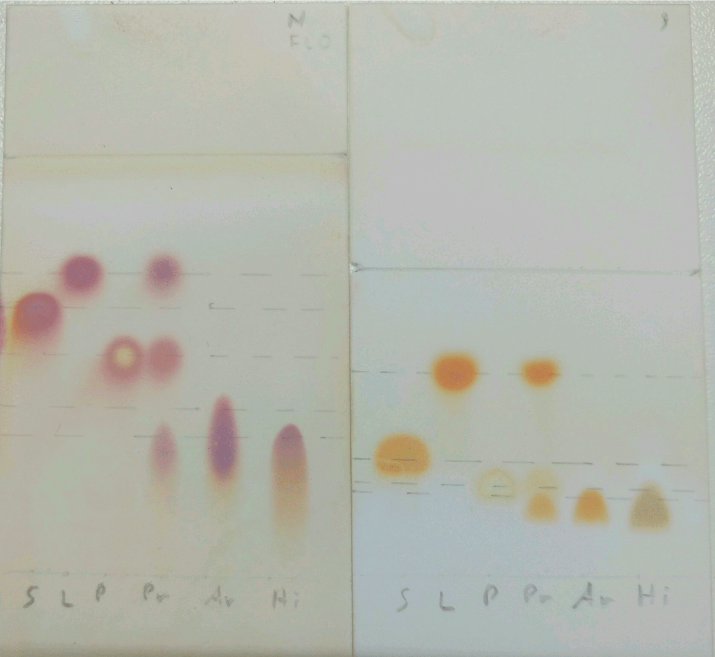
\includegraphics[scale=0.25, center]{images/test.png} 
    %\caption[Quelle: Autor]{Test}
    %\label{fig:Test}
  %\end{figure}
      